\documentclass[12pt,a4paper]{ctexart}
\usepackage{amssymb}
\usepackage{amsmath}
\usepackage{graphicx,subfig} 
\usepackage{float}
\usepackage[linesnumbered,ruled]{algorithm2e}


\title{\heiti 凸优化}
\author{2333105 宁之恒}
\date{}
\begin{document}
\maketitle

\subsection*{question1}
证明如果$\mathcal{S}_1$和$\mathcal{S}_2$是$\mathbb{R}^{m \times n}$中的凸集,那么它们的部分和
$\mathcal{S}=\{(\boldsymbol{x},\boldsymbol{y}_1+\boldsymbol{y}_2)|\boldsymbol{x} \in \mathbb{R}^m,\boldsymbol{y}_1,\boldsymbol{y}_2 \in \mathbb{R}^n,(\boldsymbol{x},\boldsymbol{y}_1) \in \mathcal{S}_1,(\boldsymbol{x},\boldsymbol{y}_2)\in \mathcal{S}_2\}$
也是凸的。

\subsection*{solve1}
欲证明$\mathcal{S}$为凸,
只需证明对于任意$(\boldsymbol{x_1},\boldsymbol{z_1}),(\boldsymbol{x_2},\boldsymbol{z_2}) \in \mathcal{S}$,$\theta \in [0,1]$有$\theta(\boldsymbol{x_1},\boldsymbol{z_1})+(1-\theta)(\boldsymbol{x_2},\boldsymbol{z_2}) \in \mathcal{S}$。
(其中$\boldsymbol{z}_1=\boldsymbol{y}_1+\boldsymbol{y}_2$,$\boldsymbol{z}_2=\boldsymbol{y}_3+\boldsymbol{y}_4$,$
(\boldsymbol{x}_1,\boldsymbol{y}_1),(\boldsymbol{x}_2,\boldsymbol{y}_3) \in \mathcal{S}_1$,$(\boldsymbol{x}_1,\boldsymbol{y}_2),(\boldsymbol{x}_2,\boldsymbol{y}_4) \in \mathcal{S}_2$)。
\begin{align*}
\theta(\boldsymbol{x_1},\boldsymbol{z_1})+(1-\theta)(\boldsymbol{x_2},\boldsymbol{z_2})
=&(\theta \boldsymbol{x}_1+(1-\theta)\boldsymbol{x}_2,\theta \boldsymbol{z}_1+(1-\theta)\boldsymbol{z}_2)\\
=&(\theta \boldsymbol{x}_1+(1-\theta)\boldsymbol{x}_2,\theta\boldsymbol{y}_1+(1-\theta)\boldsymbol{y}_3+\theta \boldsymbol{y}_2+(1-\theta)\boldsymbol{y}_4)\\
=&(\theta \boldsymbol{x}_1+(1-\theta)\boldsymbol{x}_2,\theta\boldsymbol{y}_1+(1-\theta)\boldsymbol{y}_3)\\
&\oplus(\theta \boldsymbol{x}_1+(1-\theta)\boldsymbol{x}_2,\theta \boldsymbol{y}_2+(1-\theta)\boldsymbol{y}_4)\\
=&\boldsymbol{s}_1\oplus\boldsymbol{s}_2
\end{align*}
其中$\oplus$代表部分和。\\
根据凸集的性质自然有
$(\theta \boldsymbol{x}_1+(1-\theta)\boldsymbol{x}_2,\theta\boldsymbol{y}_1+(1-\theta)\boldsymbol{y}_3)=\theta(\boldsymbol{x_1},\boldsymbol{y_1})+(1-\theta)(\boldsymbol{x}_2,\boldsymbol{y}_3)=\boldsymbol{s}_1 \in \mathcal{S}_1$,
$(\theta \boldsymbol{x}_1+(1-\theta)\boldsymbol{x}_2,\theta\boldsymbol{y}_2+(1-\theta)\boldsymbol{y}_4)=\theta(\boldsymbol{x_1},\boldsymbol{y_2})+(1-\theta)(\boldsymbol{x}_2,\boldsymbol{y}_4)=\boldsymbol{s}_2 \in \mathcal{S}_2$。
根据$\mathcal{S}$的定义,自然有$\boldsymbol{s_1}\oplus\boldsymbol{s_2} \in \mathcal{S}$,这说明$\mathcal{S}$是一个凸集。

\subsection*{question2}
对于任意$\boldsymbol{x} \in \mathbb{R}^n$,用$\boldsymbol{x}_{[i]}$表示$\boldsymbol{x}$中第$i$大的分量,即将$\boldsymbol{x}$的分量按照非升序进行排列得到下式
$\boldsymbol{x}_{[1]} \geq \boldsymbol{x}_{[2]} \geq \ldots \geq \boldsymbol{x}_{[n]}$。证明对$\boldsymbol{x}$的最大$r$个分量进行求和所得到的函数$f(x)=\sum_{i=1}^r \boldsymbol{x}_{[i]}$是凸函数。

\subsection*{solve2}
\textbf{引理}:对于$\boldsymbol{x} \in \mathbb{R}^n$,$\boldsymbol{x}=[x_1,\ldots,x_n]^T$,$\max\limits_{i}\{\boldsymbol{x}\}=\max\limits_{i}\{x_1,\ldots,x_n\}$是凸函数。
证明如下:\\
任取$\boldsymbol{x},\boldsymbol{y} \in \mathbb{R}^n$,$\theta \in [0,1]$,有
\begin{align*}
&\theta \max\limits_{i}\{\boldsymbol{x}\}+(1-\theta)\max\limits_{i}\{\boldsymbol{y}\}\\
=&\theta \max\limits_{i}\{x_1,\ldots,x_n\}+(1-\theta)\max\limits_{i}\{y_1,\ldots,y_n\}\\
=&\theta x_{[1]}+(1-\theta)y_{[1]}\\
\geq &\max\limits_{i}\{\theta x_1+(1-\theta)y_1,\ldots,\theta x_n+(1-\theta)y_n\}= \max\limits_{i}\{\theta \boldsymbol{x}+(1-\theta)\boldsymbol{y}\}
\end{align*}
其中$x_{[1]}$、$y_{[1]}$分别代表$\{x_1,\ldots,x_n\}$、$\{y_1,\ldots,y_n\}$中最大的元素。\\
接着证明比题目更强的命题:对于任意$\boldsymbol{x} \in \mathbb{R}^n$,
对$\boldsymbol{x}$的最大$r$个分量进行求和所得到的函数$f(x)=\sum\limits_{i=1}^r \boldsymbol{x}_{[i]}$\textbf{仍然}是凸函数。证明如下:\\
构造矩阵$\boldsymbol{A} \in \mathbb{R}^{C_{n}^r \times n}$,其中$C_{n}^r=\frac{n!}{r!(n-r)!}$。矩阵$A$的每一行$\boldsymbol{a}_k$由$r$个$1$和$n-r$个$0$组成,
容易证明$\boldsymbol{a}_k$有$C_{n}^r$种组合方式。令$\boldsymbol{b}=\boldsymbol{A}x$,
则$f(x)=\sum\limits_{i=1}^r \boldsymbol{x}_{[i]}=\max\limits_{k}\{\boldsymbol{b}\}$。根据\textbf{引理}可知,$\max\limits_{k}\{\boldsymbol{b}\}$
为凸函数。\\
特别的,对于非升序排列的向量$\boldsymbol{x}$,令$\boldsymbol{a}_1=[\underbrace{1,\ldots,1}_{r\text{个}1},0,\ldots,0]^T$,则
$f(x)\triangleq \max\limits_{k}\{\boldsymbol{b}\}=b_1=\boldsymbol{a}_1^T \boldsymbol{x}$同样是一个凸函数。

\subsection*{question3}
判断下列函数是否是凸函数、凹函数、拟凸函数以及拟凹函数?
\begin{itemize}
\item[(a)] 函数$f(x)=e^x-1$,定义域为$\mathbb{R}$。
\item[(b)] 函数$f(x_1,x_2)=x_1x_2$,定义域为$\mathbb{R}^2_{++}$。
\item[(c)] 函数$f(x_1,x_2)=\frac{1}{x_1x_2}$,定义域为$\mathbb{R}^2_{++}$。
\item[(d)] 函数$f(x_1,x_2)=\frac{x_1}{x_2}$,定义域为$\mathbb{R}^2_{++}$。
\item[(e)] 函数$f(x_1,x_2)=\frac{x_1^2}{x_2}$,定义域为$\mathbb{R} \times \mathbb{R}_{++}$。
\item[(f)] 函数$f(x_1,x_2)=x_1^a x_2^{1-a}$,其中$0 \leq a \leq 1$,定义域为$\mathbb{R}^2_{++}$。
\end{itemize} 

\subsection*{solve3}
容易验证,以上所有函数的定义域是凸集。并且我们通过顺序主子式讨论Hessian矩阵的正定性,在之后的证明过程中不再赘述。
\begin{itemize}
    \item[(a)] $f''(x)=e^x \geq 0$,根据图像易得其凹凸性。\\
    \textbf{结论}:是凸函数,非凹函数,是拟凸函数,是拟凹函数。
    \item[(b)] $\nabla^2f(x_1,x_2)=
    \begin{bmatrix}
        0 & 1 \\
        1 & 0
    \end{bmatrix} 
     $是不定的, 所以非凸函数,非凹函数,是拟凸函数。
    而其$\alpha$下水平集$\mathcal{C}_{\alpha}=\{(x_1,x_2) \in \mathbb{R}^2_{++} | x_1x_2\leq \alpha\}$
    不是凸集,所以非拟凸函数;其$\alpha$上水平集$\mathcal{S}_{\alpha}=\{(x_1,x_2) \in \mathbb{R}^2_{++} | x_1x_2\geq \alpha\}$
    是凸集,所以是拟凹函数。
    (这分别对应着正半轴上$xy=k$双曲线的一支所分割成的两个平面)。\\
    \textbf{结论}:非凸函数,非凹函数,非拟凸函数,是拟凹函数。
    \item[(c)] $\nabla^2f(x_1,x_2)=
    \begin{bmatrix}
        \frac{2}{x_1^3x_2} & \frac{1}{x_1^2x_2^2} \\
        \frac{1}{x_1^2x_2^2} & \frac{2}{x_1x_2^3}
    \end{bmatrix} \succ 0
    $,是凸函数,非凹函数,是拟凸函数。而其$\alpha$上水平集$\mathcal{C}_{\alpha}=\{(x_1,x_2) \in \mathbb{R}^2_{++} | x_1x_2\leq \alpha\}$
    不是凸集,所以非拟凹函数。\\
    \textbf{结论}:是凸函数,非凹函数,是拟凸函数,非拟凹函数。
    \item[(d)] $\nabla^2f(x_1,x_2)=
    \begin{bmatrix}
        0 & -\frac{1}{x_2^2} \\
        -\frac{1}{x_2^2} & \frac{2x_1}{x_2^3}
    \end{bmatrix} 
    $是不定的。所以是非凸函数,非凹函数。而其$\alpha$下水平集$\mathcal{C}_{\alpha}=\{(x_1,x_2) \in \mathbb{R}^2_{++} | \frac{x_1}{x_2}\leq \alpha\}$
    是凸集,所以是拟凸函数;而其$\alpha$上水平集$\mathcal{S}_{\alpha}=\{(x_1,x_2) \in \mathbb{R}^2_{++} | \frac{x_1}{x_2}\geq \alpha\}$
    是凸集,所以是拟凹函数(它们刚好都对应着半平面)。\\
    \textbf{结论}:非凸函数,非凹函数,是拟凸函数,是拟凹函数。
    \item[(e)] $\nabla^2f(x_1,x_2)=
    \begin{bmatrix}
        \frac{2}{x_2} & -\frac{2x_1}{x_2^2} \\
        -\frac{2x_1}{x_2^2} & \frac{2x_1^2}{x_2^3}
    \end{bmatrix} \succeq 0
    $,是凸函数,非凹函数,是拟凸函数。而其$\alpha$上水平集$\mathcal{S}_{\alpha}=\{(x_1,x_2) \in \mathbb{R}^2_{++} | \frac{x_1^2}{x_2}\geq \alpha\}$
    不是凸集,所以非拟凹函数。\\
    \textbf{结论}:是凸函数,非凹函数,是拟凸函数,非拟凹函数。
    \item[(f)]
    $
        \nabla^2f(x_1,x_2)=\left\{
        \begin{array}{ll}
        \boldsymbol{O}_{2 \times 2}, &a=1\ or\ 0\\
        \begin{bmatrix}
            a(a-1)x_1^{a-2}x_2^{1-a} & a(1-a)x_1^{a-1}x_2^{-a} \\
            a(1-a)x_1^{a-1}x_2^{-a} & a(a-1)x_1^{a}x_2^{-a-1}
        \end{bmatrix} & 0<a<1
        \end{array}
        \right.
    $
    $\nabla^2 f(x_1,x_2) \preceq 0$,非凸函数,是凹函数,是拟凹函数。
    而其$\alpha$下水平集$\mathcal{C}_{\alpha}=\{(x_1,x_2) \in \mathbb{R}^2_{++} | x_1^a x_2^{1-a}\leq \alpha\}$
    不是凸集,所以非拟凸函数。\\
    \textbf{结论}:非凸函数,是凹函数,非拟凸函数,是拟凹函数。

\end{itemize}  

\subsection*{question4}
考虑优化问题
\begin{align*}
\min_{x_1,x_2} \ &f_0(x_1,x_2) \\
\rm{s.t.}\  &2x_1+x_2 \geq 1\\
          & x_1+3x_2 \geq 1\\
          &x_1 \geq 0,x_2 \geq 0
\end{align*}
对其可行集进行概述。对下面每个目标函数,给出最优解和最优值。
\begin{itemize}
    \item[(a)] $f_0(x_1,x_2)=x_1+x_2$
    \item[(b)] $f_0(x_1,x_2)=-x_1-x_2$
    \item[(c)] $f_0(x_1,x_2)=x_1$
    \item[(d)] $f_0(x_1,x_2)=\max\{x_1,x_2\}$
    \item[(e)] $f_0(x_1,x_2)=x_1^2+9x_2^2$
\end{itemize}  

\subsection*{solve4}
构造拉格朗日函数$L(x_1,x_2,\boldsymbol{\lambda})=f_0(x_1,x_2)+\lambda_1(1-2x_1-x_2)
+\lambda_2(1-x_1-3x_2)+\lambda_3(-x_1)+\lambda_4(-x_2)$,其中$\boldsymbol{\lambda} \geq 0$
对于上述五个函数$f_0(x_1,x_2)$,
容易验证它们都是关于$\boldsymbol{x}=[x_1,x_2]^T$的凸函数。
则$\nabla_{\boldsymbol{x}} L(x_1,x_2,\boldsymbol{\lambda})=\nabla f_0(x_1,x_2)+(-2\lambda_1-\lambda_2-\lambda_3,-\lambda_1-3\lambda_2-\lambda_4)$。\\
并且给出满足以下凸问题的KKT条件:
\begin{align*}
\left \{
\begin{array}{ll}
    &2x_1+x_2 \geq 1,x_1+3x_2 \geq 1,x_1 \geq 0,x_2 \geq 0\\
    &\lambda_1,\lambda_2,\lambda_2,\lambda_4 \geq 0\\
    & \lambda_1 (1-2x_1-x_2)=0,\lambda_2(1-x_1-3x_2)=0,\lambda_3(-x_1)=0,\lambda_4(-x_2)=0\\
    & \nabla_{\boldsymbol{x}}L(x_1,x_2,\boldsymbol{\lambda})=0\\
\end{array}
\right.
\end{align*}
先作简单的分析,在二维平面内的仿射约束只会重合或两两交于一点。这说明了互补松弛条件中,
$\lambda_1,\lambda_2,\lambda_3,\lambda_4$最多存在两个同时为0。
\begin{itemize}
    \item[(a)] $f_0(x_1,x_2)=x_1+x_2$,最优解为$(x_1,x_2)=(\frac{2}{5},\frac{1}{5})$,最优值为$\frac{2}{3}$
    \item[(b)] $f_0(x_1,x_2)=-x_1-x_2$,不存在最优解与最优值(最优解为$(+\infty,+\infty)$最优值为$-\infty$)
    \item[(c)] $f_0(x_1,x_2)=x_1$,最优解为$(x_1,x_2)=(0,x_2)$,其中$x_2 \geq 1$,最优值为$0$
    \item[(d)] $f_0(x_1,x_2)=\max\{x_1,x_2\}$,最优解为$(x_1,x_2)=(\frac{1}{3},\frac{1}{3})$,最优值为$\frac{1}{3}$
    \item[(e)] $f_0(x_1,x_2)=x_1^2+9x_2^2$,最优解为$(x_1,x_2)=(\frac{1}{2},\frac{1}{6})$,最优值为$\frac{1}{2}$
\end{itemize}  

\subsection*{question5}
给出下面每个线性规划(LP)的显式解。
\begin{itemize}
    \item[(a)] 在仿射集合上极小化线性函数。
    \begin{align*}
        \min\limits_{\boldsymbol{x}} \ &\boldsymbol{c}^T\boldsymbol{x} \\
        \rm{s.t.}\  &\boldsymbol{Ax}=\boldsymbol{b}
    \end{align*}
    \item[(b)] 在半空间上极小化线性函数。
    \begin{align*}
        \min\limits_{\boldsymbol{x}} \ &\boldsymbol{c}^T\boldsymbol{x} \\
        \rm{s.t.}\  &\boldsymbol{a}^T \boldsymbol{x} \leq b
    \end{align*}
    其中$\boldsymbol{a} \neq \boldsymbol{0}$。
    \item[(c)] 在矩阵上极小化线性函数。
    \begin{align*}
        \min\limits_{\boldsymbol{x}} \ &\boldsymbol{c}^T\boldsymbol{x} \\
        \rm{s.t.}\  &\boldsymbol{l} \preceq \boldsymbol{x} \preceq  \boldsymbol{u}
        \end{align*}
    其中 $\boldsymbol{l}$和$\boldsymbol{u}$满足$\boldsymbol{l} \preceq \boldsymbol{u}$。
    \item[(d)] 在概率单纯形上极小化线性函数。
    \begin{align*}
        \min\limits_{\boldsymbol{x}} \ &\boldsymbol{c}^T\boldsymbol{x} \\
        \rm{s.t.}\  &\boldsymbol{1}^T \boldsymbol{x} =1 \\
                    & \boldsymbol{x}\succeq \boldsymbol{0}
        \end{align*}
\end{itemize}  

\subsection*{solve5}
由于它们都是线性规划的问题,满足weak-slater's condition。那么其
对偶问题的最优解则为原问题的最优解。
\begin{itemize}
\item[(a)] 
\begin{align*}
    \min\limits_{\boldsymbol{x}} \ &\boldsymbol{c}^T\boldsymbol{x} \\
    \rm{s.t.}\  &\boldsymbol{Ax}=\boldsymbol{b}
\end{align*}
构造拉格朗日函数$L(\boldsymbol{x},\boldsymbol{\nu})=
\boldsymbol{c}^T\boldsymbol{x}+\boldsymbol{\nu}^T(\boldsymbol{Ax}-\boldsymbol{b})$,其中$\boldsymbol{\nu} \in \mathbb{R}^n$,
对其求偏导可得$\nabla_{\boldsymbol{x}} L(\boldsymbol{x},\boldsymbol{\nu})=\boldsymbol{c}+\boldsymbol{ A}^T \boldsymbol{\nu}$。\\
若$\boldsymbol{Ax}=\boldsymbol{b}$无解,即$\boldsymbol{b} \notin \mathcal{R}(\boldsymbol{A})$:
\begin{align*}
g(\boldsymbol{\nu})=+\infty
\end{align*}
若其有解:
\begin{align*}
g(\boldsymbol{\nu})=\left \{
\begin{array}{ll}
\boldsymbol{c}^T (\boldsymbol{A})^{+}\boldsymbol{b} &\boldsymbol{c}+\boldsymbol{A}^T \boldsymbol{\nu}=\boldsymbol{0}\\
-\infty &\rm{otherwise}
\end{array}
\right.
\end{align*}
其中$(\cdot)^+$是广义逆运算。\\
综上,对偶问题为:
\begin{align*}
    \max\limits_{\boldsymbol{\nu}} g(\boldsymbol{\nu})=\left \{
    \begin{array}{ll}
    +\infty &\boldsymbol{b} \notin R(\boldsymbol{A})\\
    \boldsymbol{c}^T (\boldsymbol{A})^{+}\boldsymbol{b} &\boldsymbol{c}+\boldsymbol{A}^T \boldsymbol{\nu}=\boldsymbol{0}\\
    -\infty &\rm{otherwise}
    \end{array}
    \right.
    \end{align*}
其中$\boldsymbol{\nu}\in \mathbb{R}^n$。\\
则显示解为:
\begin{align*}
    \min\limits_{\boldsymbol{x}} \boldsymbol{c}^T\boldsymbol{x}
    =\left \{
    \begin{array}{ll}
    +\infty &\boldsymbol{b} \notin R(\boldsymbol{A})\\
    \boldsymbol{c}^T (\boldsymbol{A})^{+}\boldsymbol{b} &\boldsymbol{c}+\boldsymbol{A}^T \boldsymbol{\nu}=\boldsymbol{0}\\
    -\infty &\rm{otherwise}
    \end{array}
    \right.
    \end{align*}
\item[(b)]
\begin{align*}
    \min\limits_{\boldsymbol{x}} \ &\boldsymbol{c}^T\boldsymbol{x} \\
    \rm{s.t.}\  &\boldsymbol{a}^T \boldsymbol{x} \leq b
\end{align*}
构造拉格朗日函数$L(\boldsymbol{x},\lambda)=
\boldsymbol{c}^T\boldsymbol{x}+\lambda(\boldsymbol{a}^T\boldsymbol{x}-b)$,其中$\lambda \geq 0$,
对其求偏导可得$\nabla_x L(\boldsymbol{x},\lambda)=\boldsymbol{c}+\lambda \boldsymbol{a} $,则对偶问题为:
\begin{align*}
    \max\limits_{\boldsymbol{\lambda}}&\ g(\lambda)=\left \{
    \begin{array}{ll}
    -\lambda b &\boldsymbol{c}+\lambda \boldsymbol{a} =0\\
    -\infty &\rm{otherwise}
    \end{array}
    \right.\\
    \rm{s.t.}&\ \lambda \geq 0
    \end{align*}
显示解为:
\begin{align*}
    \min\limits_{\boldsymbol{x}} \boldsymbol{c}^T\boldsymbol{x}
    =\left \{
    \begin{array}{ll}
    -\lambda b &\boldsymbol{c}+\lambda \boldsymbol{a} =0\\
    -\infty &\rm{otherwise}
    \end{array}
    \right.
    \end{align*}
\item[(c)] 
\begin{align*}
    \min\limits_{\boldsymbol{x}} \ &\boldsymbol{c}^T\boldsymbol{x} \\
    \rm{s.t.}\  &\boldsymbol{l} \preceq \boldsymbol{x} \preceq  \boldsymbol{u}
    \end{align*}
其中 $\boldsymbol{l}$和$\boldsymbol{u}$满足$\boldsymbol{l} \preceq \boldsymbol{u}$。

构造拉格朗日函数$L(\boldsymbol{x},\boldsymbol{\lambda})=
\boldsymbol{c}^T\boldsymbol{x}+\boldsymbol{\lambda}_1^T(\boldsymbol{l}-\boldsymbol{x})+\boldsymbol{\lambda}_2^T(\boldsymbol{x}-\boldsymbol{u})$,其中$\boldsymbol{\lambda}_1,\boldsymbol{\lambda}_2 \succeq \boldsymbol{0}$,
对其求偏导可得$\nabla_x L(\boldsymbol{x},\boldsymbol{\lambda})=\boldsymbol{c}-\boldsymbol{\lambda}_1+\boldsymbol{\lambda}_2$,则:
\begin{align*}
    g(\boldsymbol{\lambda})=
    \boldsymbol{\lambda}_1^T\boldsymbol{l}-\boldsymbol{\lambda}_2^T \boldsymbol{u} ,\quad &\boldsymbol{c}-\boldsymbol{\lambda}_1+\boldsymbol{\lambda}_2=\boldsymbol{0}
\end{align*}
此时包含两个未知变量$\boldsymbol{\lambda}_1$、$\boldsymbol{\lambda}_2$,无法得到显示解。\\
令$\boldsymbol{c}=[c_1,\ldots,c_n]^T$,如果$c_i<0$,则$x_i=l_i$;如果$c_i>0$,则$x_i=u_i$;如果$c_i=0$,则$x_i$为符合约束条件的任意值都可以。那么显示解为:
\begin{align*}
\min\limits_{\boldsymbol{x}} \boldsymbol{c}^T\boldsymbol{x}=\sum\limits_{c_i\geq 0,c_i \in \boldsymbol{c}}c_i l_i+\sum\limits_{c_j<0,c_j \in \boldsymbol{c}}c_j u_j
\end{align*}
\item[(d)] 
    \begin{align*}
        \min\limits_{\boldsymbol{x}} \ &\boldsymbol{c}^T\boldsymbol{x} \\
        \rm{s.t.}\  &\boldsymbol{1}^T \boldsymbol{x} =1 \\
                    & \boldsymbol{x}\succeq \boldsymbol{0}
        \end{align*}
构造拉格朗日函数$L(\boldsymbol{x},\boldsymbol{\lambda},\nu)=
\boldsymbol{c}^T\boldsymbol{x}+v(\boldsymbol{1}^T\boldsymbol{x}-\boldsymbol{1})+\boldsymbol{\lambda}^T(-\boldsymbol{x})$,其中$\nu \in \mathbb{R},\boldsymbol{\lambda} \succeq \boldsymbol{0}$,
对其求偏导可得$\nabla_x L(\boldsymbol{x},\boldsymbol{\lambda},\nu)=\boldsymbol{c}+\nu \boldsymbol{1}-\boldsymbol{\lambda}$,则:
\begin{align*}
    g(\boldsymbol{\lambda},\nu)=
    -\nu,\quad &\boldsymbol{c}+\nu \boldsymbol{1}-\boldsymbol{\lambda}=\boldsymbol{0}
\end{align*}
此时包含两个未知变量$\nu$、$\boldsymbol{\lambda}$,无法得到显示解。\\
令$\boldsymbol{c}=[c_1,\ldots,c_n]^T$,把$\{c_1,\ldots,c_n\}$按照升序排列变成$\hat{\boldsymbol{c}}=[c_{[1]},\ldots,c_{[n]}]$。
此时令$\boldsymbol{x}=[1,0,\ldots,0]^T$,则$\hat{\boldsymbol{c}}^T\boldsymbol{x}$则为目标函数的最小值,其值为$c_{[1]}$。那么:
\begin{align*}
\min\limits_{\boldsymbol{x}} \boldsymbol{c}^T\boldsymbol{x}=\min\limits_{c_i}{\boldsymbol{c}}
\end{align*}
\end{itemize} 

\subsection*{question6}
给出如下优化函数式
\begin{align*}
    \min\limits_{\boldsymbol{x}} \ &\boldsymbol{c}^T\boldsymbol{x} \\
    \rm{s.t.}\  &\boldsymbol{Ax}=\boldsymbol{b}\\
                & \boldsymbol{x} \succeq \boldsymbol{0}
\end{align*}
写出其Lagrange方程,写出其对偶函数解。

\subsection*{solve6}
构造拉格朗日函数$L(\boldsymbol{x},\boldsymbol{\lambda},\boldsymbol{\nu})=
\boldsymbol{c}^T\boldsymbol{x}+\boldsymbol{\nu}^T(\boldsymbol{Ax}-\boldsymbol{b})+\boldsymbol{\lambda}^T(-\boldsymbol{x})$,其中$\boldsymbol{\nu} \in \mathbb{R}^n,\boldsymbol{\lambda} \succeq \boldsymbol{0}$,
对其求偏导可得$\nabla_{\boldsymbol{x}} L(\boldsymbol{x},\boldsymbol{\lambda})=\boldsymbol{c}+\boldsymbol{ A}^T \boldsymbol{\nu}-\boldsymbol{\lambda}$。\\
若$\boldsymbol{Ax}=\boldsymbol{b}$无解,即$\boldsymbol{b} \notin \mathcal{R}(\boldsymbol{A})$:
\begin{align*}
g(\boldsymbol{\lambda},\boldsymbol{\nu})=+\infty
\end{align*}
若其有解:
\begin{align*}
    g(\boldsymbol{\lambda},\boldsymbol{\nu})=\left \{
    \begin{array}{ll}
    -\boldsymbol{\nu}^T \boldsymbol{b} &\boldsymbol{c}+\boldsymbol{ A}^T \boldsymbol{\nu}-\boldsymbol{\lambda}=\boldsymbol{0}\\
    -\infty &\rm{otherwise}
    \end{array}
    \right.
\end{align*}
综上,对偶函数解析式为:
\begin{align*}
    g(\boldsymbol{\lambda},\boldsymbol{\nu})=\left \{
    \begin{array}{ll}
    +\infty &\boldsymbol{b} \notin \mathcal{R}(\boldsymbol{A})\\
    -\boldsymbol{\nu}^T \boldsymbol{b} &\boldsymbol{c}+\boldsymbol{ A}^T \boldsymbol{\nu}-\boldsymbol{\lambda}=\boldsymbol{0}\\
    -\infty &\rm{otherwise}
    \end{array}
    \right.
\end{align*}

\subsection*{question7}
对下述问题,给出其对偶函数解析式,并给出其最优值的下界。
\begin{align*}
    \min\limits_{\boldsymbol{x}} \ &\boldsymbol{x}^T\boldsymbol{W}\boldsymbol{x} \\
    \rm{s.t.}\  &x_i^2=1,i=1,\ldots,n
\end{align*}
其中$\boldsymbol{W} \in \mathbb{S}^n$,$\boldsymbol{x}=[x_1,\ldots,x_n]^T$。


\subsection*{solve7}
由于可行集$\rm{dom}f$不是凸集,并且目标函数$f_0(\boldsymbol{x})$不是凸函数,所以这不是一个凸问题。\\
构造拉格朗日函数$L(\boldsymbol{x},\boldsymbol{\nu})=\boldsymbol{x}^T\boldsymbol{W}\boldsymbol{x}+\sum\limits_{i=1}^n \nu_i(x_i^2-1)$,
其中$\boldsymbol{\nu}=[\nu_1,\ldots,\nu_n]^T$。对矩阵$\boldsymbol{W}$进行行分块$[\boldsymbol{w}_1,\ldots,\boldsymbol{w}_n]^T$,对$\boldsymbol{x}$的每个分量求偏导:
\begin{align*}
\frac{\partial L(\boldsymbol{x},\boldsymbol{\nu})}{\partial x_i}=&2\boldsymbol{w}_i^T\boldsymbol{x}+2\nu_i x_i\\
                                                              =&2w_{i1}x_1+\cdots+(2w_{ii}x_i+2\nu_i)x_i+\cdots+2w_{in}x_n     
\end{align*}
令$\frac{\partial L(\boldsymbol{x},\boldsymbol{\nu})}{\partial x_1}=\cdots=\frac{\partial L(\boldsymbol{x},\boldsymbol{\nu})}{\partial x_n}=0$,
等价于求解矩阵方程组$\boldsymbol{Sx}=\boldsymbol{0}$,
其中$\boldsymbol{S}=
\begin{pmatrix}
2w_{11}+2v_1 & 2w_{12} &\cdots &2w_{1n} \\
2w_{21} &2w_{22}+2v_2 & \cdots &2w_{2n}\\
\vdots &\vdots &\ddots &\vdots\\
2w_{n1} &2w_{n2} & \cdots & 2w_{nn}+2v_n
\end{pmatrix}=2\boldsymbol{W}+2\rm{diag}\{\boldsymbol{\nu}\}
$。\\
若方程组有解,即$\boldsymbol{Wx}=-\rm{diag}\{\boldsymbol{\nu}\} \boldsymbol{x}$
所以,对偶函数为:
\begin{align*}
g(\boldsymbol{\nu})=&\boldsymbol{x}^T\boldsymbol{W}\boldsymbol{x}=\sum\limits_{i=1}^n -\nu_i x_i^2=-\boldsymbol{\nu}^T\boldsymbol{1}
\end{align*}
若方程组无解,根据$\boldsymbol{W}$的任意性,对偶函数为:
\begin{align*}
    g(\boldsymbol{\nu})= -\infty
\end{align*}
综上,对偶函数为:
\begin{align*}
g(\boldsymbol{\nu})=\left \{
\begin{array}{ll}
    -\boldsymbol{\nu}^T\boldsymbol{1} & \boldsymbol{Sx}=\boldsymbol{0}\\
    -\infty  & \rm{otherwise}
\end{array}
\right .
\end{align*}
对偶问题为:
\begin{align*}
\max\limits_{\boldsymbol{\nu}}\ g(\boldsymbol{\nu})=\left \{
\begin{array}{ll}
    -\boldsymbol{\nu}^T\boldsymbol{1} & \boldsymbol{Sx}=\boldsymbol{0}\\
    -\infty  & \rm{otherwise}
\end{array}
\right .
\end{align*}
其中$\boldsymbol{x}=[x_1,\ldots,x_n]^T$,并且$x_i^2=1,i=1,\ldots,n$。
$\boldsymbol{S}=2\boldsymbol{W}+\rm{diag}\{\boldsymbol{\nu}\}$。\\
由于最小值为$-\infty$没有任何意义,因此根据对偶问题给出的一个
较优的下界为$-\boldsymbol{\nu}^T\boldsymbol{1}$。

\subsection*{question8}
考虑优化问题
\begin{align*}
    \min\limits_{x}\  &x^2+1\\
    \rm{s.t.}\  &(x-2)(x-4) \leq 0
\end{align*}
其中变量$x \in \mathbb{R}$。
\begin{itemize}
    \item[(a)] 分析原问题。求解可行集,最优值以及最优解。
    \item[(b)] Lagrange函数以及对偶函数。绘制目标函数根据$x$变化的图像。在同一幅图中,标出可行集,最优点及最优值,选择一些正的Lagrange乘子$\lambda$,
    绘出Lagrange函数$L(x,\lambda)$关于x的变化曲线。利用图像,证明下界性质(即对任意$\lambda \geq 0$,$p^* \geq \inf_xL(x,\lambda)$)。
    推导Lagrange对偶函数g并大致描绘其图像。
    \item[(c)]Lagrange对偶问题。描述对偶问题,证明它是一个凹极大化问题。求解对偶最优值以及对偶最优解$\lambda^*$。此时强对偶性是否成立?
\end{itemize}
\newpage


\subsection*{solve8}
\begin{itemize}
    \item[(a)] 这是一个二次约束二次规划的问题。
    可行集为$x \in [2,4]$,最优值为$5$,最优解为$x=2$。
    \item[(b)]
    1.目标函数$f_0(x)$\\
    图 \ref{f_0(x)}给出了函数$f_0(x)=x^2+1$的图像。\\
    \begin{figure}[!h] %h表示就在此处插入。
        \centering % 居中
        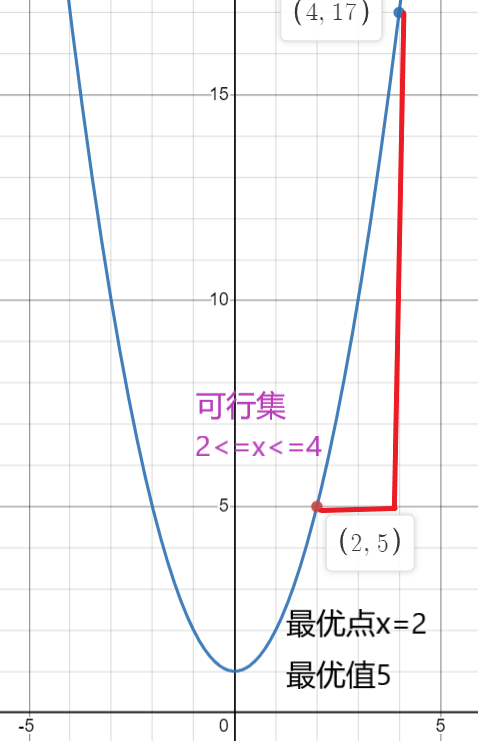
\includegraphics[scale=0.5]{f_0(x).png} %在tex所在文件夹下面创建一个名为figs的文件夹,并把所有要用的照片放这里。当然你也可以选择使用绝对路径。
        \caption{$f_0(x)=x^2+1$函数图像}
        \label{f_0(x)} % 为每个图片设置一个标识
    \end{figure}
    2.拉格朗日函数$L(x,\lambda)$\\
    构造拉格朗日函数$L(x,\lambda)=x^2+1+\lambda(x-2)(x-4)$,其中$\lambda \geq 0$。对$x$求偏导可得:
    \begin{align}
    \frac{\partial{L(x,\lambda)}}{\partial x}=2x+\lambda(2x-6) \label{qiudao}
    \end{align}
    图\ref{拉格朗日函数}给出了拉格朗日函数$L(x,\lambda)$的图像。若$\lambda \leq 2$,
    $\inf\limits_{x} L(x,\lambda) \leq 5=p^*$;若$\lambda > 2$,$\inf\limits_{x} L(x,\lambda) < 5=p^*$。
    这便说明了$\inf\limits_{x} L(x,\lambda) \leq p^*$。\\
    \begin{figure}[!h]
        \centering
        %\includegraphics[width=3in]{fig5}
        \subfloat[$L(x,0.5)$]{
            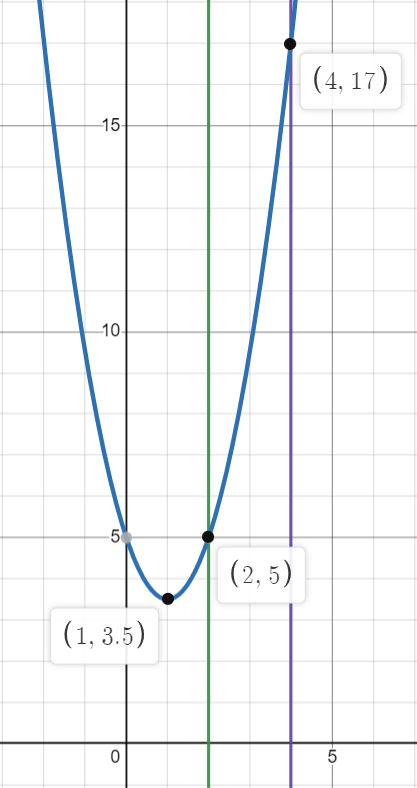
\includegraphics[scale=0.5]{L(x,0.5).png}}
        \subfloat[$L(x,2)$]{
            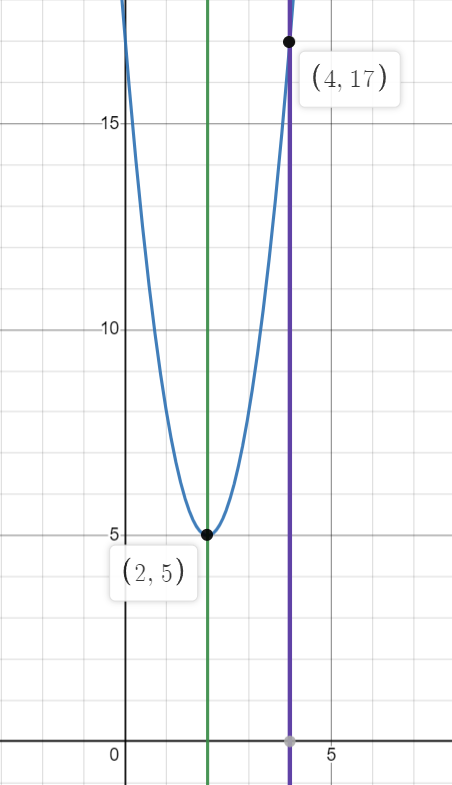
\includegraphics[scale=0.5]{L(x,2).png}}
        \\
        \subfloat[$L(x,6)$]{
            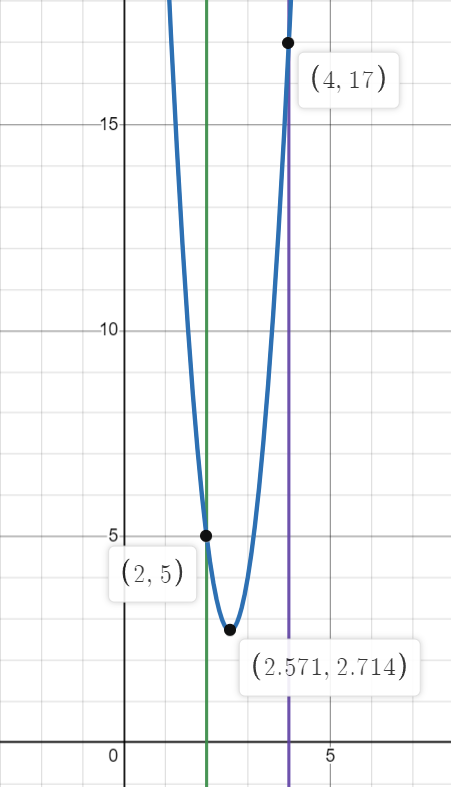
\includegraphics[scale=0.5]{L(x,6).png}}
        \subfloat[$L(x,\frac{\sqrt{85}+9}{2})$]{
            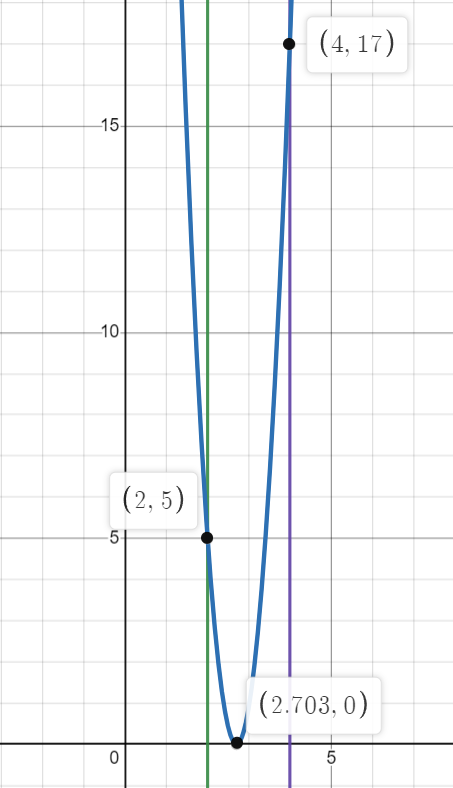
\includegraphics[scale=0.5]{L(x,x_0).png}}
        \caption{$L(x,\lambda)$函数图像}
        \label{拉格朗日函数}
    \end{figure}
    3.对偶函数$g(\lambda)$\\
    令式\eqref{qiudao}=0,可得$x=\frac{3\lambda}{1+\lambda}$,则对偶函数$g(\lambda)$为:
    \begin{align}
        g(\lambda)&=(\frac{3\lambda}{1+\lambda})^2+1+\lambda(\frac{3\lambda}{1+\lambda}-2)(\frac{3\lambda}{1+\lambda}-4) \notag \\
                                &=\frac{-\lambda^3+8\lambda^2+10\lambda+1}{(\lambda+1)^2} \label{对偶函数g表达式}
    \end{align}
    式\eqref{对偶函数g表达式}给出了对偶函数g的表达式,图\ref{对偶函数g}给出了对偶函数g的大致图像。
    \begin{figure}[!h] %h表示就在此处插入。
        \centering % 居中
        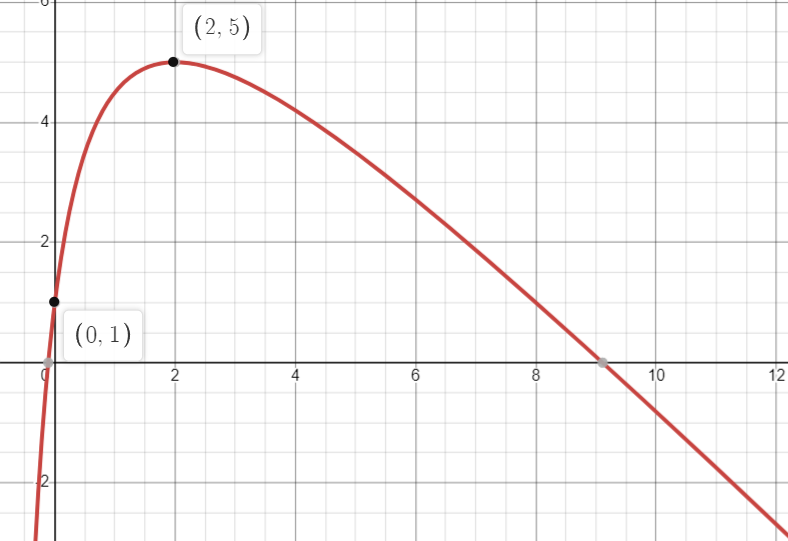
\includegraphics[scale=0.5]{g(lambda).png} %在tex所在文件夹下面创建一个名为figs的文件夹,并把所有要用的照片放这里。当然你也可以选择使用绝对路径。
        \caption{$\mathrm{g}$函数图像}
        \label{对偶函数g} % 为每个图片设置一个标识
        \end{figure}
    \item[(c)]对偶问题是:
    \begin{align*}
        \max\  &\frac{-\lambda^3+8\lambda^2+10\lambda+1}{(\lambda+1)^2}\\
        \rm{s.t.}\  &\lambda \geq 0
    \end{align*}
    对$g(\lambda)$求导,并令其等于$0$,可得
    $\lambda=2$。并且$g''(\lambda) \leq 0$恒成立,当且仅当$\lambda=2$时,$g''(\lambda)=0$,这说明了它是一个凹极大化问题。
    此时对偶问题取到最大值$d^*=g(\lambda)_{\max}=g(2)=5$,与原问题的最优值相同,
    这表明了$p^*=d^*$,则强对偶成立。
\end{itemize}
\end{document}
